% Chapter 8

\chapter{Conclusion} % Write in your own chapter title
\label{Chapter8}
\lhead{Chapter 8. \emph{Conclusion}} % Write in your own chapter title to set the page header

\section{Introduction}

The immune response to HTLV-I infection has remained an intriguing and difficult area of research for the 30 years since its discovery and classification. Why approximately 95\% of individuals who are infected with the virus remain asymptomatic and the remainder develop either debilitating inflammatory conditions (e.g.~HAM/TSP) or an aggressive T-cell lymphoma (ATL) is still not fully understood. The immune response to HTLV-I infection includes cytotoxic T lymphocytes (CTLs), antibodies, T\subscript{reg} cells and natural killer (NK) cells (\sref{chapter2/pathogenesis}). However among these adaptive immune responses, it is the CTL response that is the most important determinant of disease and proviral load.

The conflicting results of the role of CTLs (or CD8$^+$ T cells) in controlling HTLV-I infection has painted a confused picture of this arm of the immune response. On the one hand, the protective effect of a strong CD8$^+$ T cell response has been demonstrated by selection pressure on the dominant target antigen, Tax \citep{Niewiesk1994, Kubota2007}, host genetics \citep{Jeffery1999, Jeffery2000, Vine2002} and gene expression microarrays \citep{Vine2004}. Contrary to these results, the effect of HTLV-I-specific CD8$^+$ T cell frequency has been ambiguous, with different groups reporting little effect of frequency on proviral load \citep{Parker1992, Parker1994} and some reporting a positive correlation with proviral load \citep{Kubota2000, Wodarz2001}.

These data has led to the hypothesis that it is the quality of the virus-specific CTLs, and not their frequency, that determines their effectiveness in controlling viral load and the risk of associated disease \citep{Nowak1996}. This quality has been defined by a mathematical model of CTL-mediated lysis \citep{Asquith2005a} and has yielded the observation that approximately 35\% of the between-individual variation in proviral load can be explained by variation in their CD8$^+$ T cell lytic efficiency \citep{Asquith2005a, Kattan2009}.

So what is the functional basis of this variation in CD8$^+$ T cell lysis efficiency? The are a number of possibilites that have been investigated: variation in the sensitivity of CD8$^+$ T cells to antigen concentration (``functional avidity'' \citep{Kattan2009}), the ability of HTLV-I-specific CD8$^+$ T cells to respond in multiple ways to antigen (``polyfunctionality'' \citep{Bangham2009}) and the role of regulatory T cells in the CTL response \citep{Toulza2008}. However, the focus of my PhD was the observation of the protective effect of the HLA class I alleles \emph{A*02} and \emph{Cw*08} and the detrimental effect of \emph{B*54} \citep{Jeffery1999}, as well as the overall protective effect of HLA class I heterozygosity \citep{Jeffery2000}.

This variation in HLA class I effect across different alleles in terms of proviral load and the risk of associated disease suggested two observations :

\begin{enumerate}[(i)]
\item The association between HLA class I and proviral load and disease status in HTLV-I infection was - given the unequivocal function of HLA class I to display viral antigen to CTLs - the strongest evidence that CTL efficiency controls HTLV-I infection.
\item The functional difference between protective and detrimental HLA class I alleles could be understood by studying the viral epitopes that bind to these alleles.
\end{enumerate}

From this information, we formulated the following structure to try and understand the underlying mechanism of HLA class I protection:

\begin{enumerate}[(a)]
\item Refine and, if possible, improve upon existing knowledge of the associations between HLA class I alleles and markers of HTLV-I infection.
\item Rigorously test existing epitope prediction software to predict the HTLV-I epitopes that bind to the HLA class I alleles of interest.
\item Use this information to test hypotheses about the epitope properties of protective and detrimental alleles.
\item Model the CD8$^+$ T cell response in terms of its rate of lysis of infected CD4$^+$ T cells.
\item Further understand the role of CTLs and NK cells in HTLV-I infection.
\end{enumerate}

\section{A Summary of Results by Chapter}

\subsection{Refining HLA class I Allele Associations}

\cref{Chapter3} built upon the conclusions of the series of papers by Jefferys \emph{et al.} \citep{Jeffery1999, Jeffery2000} detailing the HLA class I associations with proviral load and the risk of HAM/TSP in HTLV-I infection. The conclusions of these papers can be summarised as follows:

\begin{enumerate}[(i)]
\item The presence of \emph{HLA-A*02} is associated with a lower risk of HAM/TSP and a reduced proviral load in aymptomatic carriers of HTLV-I (but not in HAM/TSP individuals).
\item Independent of the \emph{HLA-A*02} effect, the presence of \emph{HLA-Cw*08} is associated with a lower risk of HAM/TSP and a reduced proviral load in aymptomatic carriers of HTLV-I (but not in HAM/TSP individuals).
\item \emph{HLA-B*054} is associated with an increased risk of HAM/TSP and a higher proviral load in HAM/TSP patients (but not in asymptomatic carriers).
\item Individals who are heterozygous at all three HLA class I loci have a lower proviral load than those who are homozygous at one or more loci.
\end{enumerate}

Our goal was to reanalyse this data and test for any further associations. We wanted to increase the pool of statistically significant protective and detrimental alleles, which would provide us with greater power in the analysis of their epitopes. We used a combination of Mann-Whitney U tests, $\chi^2$ analysis and a novel ranking test (\sref{chapter3/methods}). This analysis suggested other HLA class I alleles could be associated with HTLV-I infection outcome (e.g.~\fref{chapter3/figureRobust}). However, these associations did not prove significant using the the data of the Kagoshima Cohort (\sref{chapter3/kagoshima}).

\subsection{Rescaling in Epitope Prediction}

The initial goal of \cref{Chapter4} was to verify epitope prediction software for our use in predicting HTLV-I epitopes. Based on our preliminary analysis, we decided to focus on the subject of rescaling predicted binding affinities - a normalization procedure built on the assumption that different HLA class I molecules will bind to the same number of viral peptides. We used a combination of ROC curve and ranking analysis (\sref{chapter4/results}) to show that, when comparing predicted binding affinitities between alleles, non-rescaled affinities are more accurate for epitope discovery. We incorporated these results into a web-based epitope prediction server (Metaserver, \sref{chapter4/results/metaserver}) and our analysis of rescaling has been verified and acknowledged by other members of the epitope prediction community \citep{Stranzl2010}.

\subsection{Using Predicted Binding Affinities}

In \cref{Chapter6}, we used epitope prediction software to define the predicted epitopes of HTLV-I. We defined our approach to understanding the basis of HLA class I protection in terms of specificity i.e.~is it advantageous (in terms of proviral load and risk of HAM/TSP) to possess alleles that bind strongly to specific HTLV-I proteins? In order to test this, we built upon a novel ranking method by Borghans \emph{et al.} \citep{borghans2007} for the study of HIV epitopes. Our method defined the strength of binding of 9-mer peptides from a specific HTLV-I protein in terms of their rank binding strength compared to every other 9-mer peptide in the HTLV-I proteome. Using this method, along with raw predicted binding affinities and the SIR metric (\sref{appendixc/sir}), and also 2 independent methods of epitope prediction (Metaserver and Epipred, \sref{chapter5/MethPred}), we reached the following conclusions:

\begin{enumerate}[(1)]
\item HLA Class I alleles previously associated with reduced proviral load and HAM/TSP prevalence (HLA-A*02 and -Cw*08) were predicted to bind epitopes from the viral protein HBZ significantly more strongly than an allele associated with increased proviral load and HAM/TSP prevalence (HLA-B*54).
\item Asymptomatic carriers had a HLA class I genotype that predisposed them to bind epitopes from HBZ significantly more strongly than HAM/TSP patients. This result remained significant even when all individuals who possessed \gene{A*02}, \gene{B*54} and/or \gene{Cw*08} were excluded from the cohort.
\item Individuals whose HLA class I genotype predisposed them to strongly bind HBZ epitopes had a significantly reduced proviral load. This result was independent of the disease association reported above.
\item Across all HTLV-I proteins, those proteins that were preferentially targeted by asymptomatic carriers were those associated with a greater reduction in proviral load when bound.
\item HBZ-specific CD8$^+$ cells were detectable by IFN$\gamma$ ELISpot in fresh PBMC from HTLV-I infected individuals.
\end{enumerate}

The importance of HBZ in inhibiting expression of other HTLV-I genes \citep{Gaudray2002, Li2009} and in promoting the proliferation of infected T-lymphocytes \citep{Satou2006} certainly complemented our findings that the protein is an important target for the host immune system. The recent observation, however, that HBZ-specific CTLs could not lyse HTLV-I infected cells in ATL patients had cast some doubt on this theory \citep{Suemori2009}. In response to this data, our laboratory (Aileen Rowan) has shown that HBZ-specific CD8$^+$ cells are detectable by a CD107a degranulation assay (as an alternative to IFN$\gamma$ ELISpot, mentioned above). We also showed that naturally infected cells from asymptomatic carriers and HAM/TSP patients are susceptible to lysis by HBZ-specific CTLs. The difference in susceptibility between non-leukaemic and ATL patients to HBZ-specific CD8$^+$ cells may be because ATL cells are inherently harder to kill and/or express lower levels of HBZ (B.~Asquith, pers.~comm.).

It was also interesting to compare the ranking of proteins in terms of proviral load and disease risk (\sref{chapter6/resultsProt}) and the immunodominance hierarchy established by Goon \emph{et al.} \citep{Goon2004}. The immunodominance hierarchy ranked the HTLV-I proteins in terms of the frequency of protein-specific CD8$^+$ T cell responses. This hierarchy of proteins (highest to lowest frequency: Tax, Pol, Env, Gag, Rof, Tof, Pro, Rex) beared no relationship to our rank order of protective immune responses \tref{chapter6/table2HypothRank}. This suggested again that immunodominance, as we found with Tax, was not necessarily related to protection in terms of targeting specific proteins in HTLV-I.   

The relationship between Tax, as the immunodominant target, and HBZ is becoming more apparent through results such as those above. The data suggests that HBZ is important during the chronic stage of infection, where Tax expression is suppressed and is thus not presented to the immune system. Tax expression then increases to drive short phases of rapid expansion of infected T lymphocytes (C.~ Bangham, pers.~comm.). Work is ongoing in our laboratory to test hypotheses generated from this relationship.

\subsection{Understanding CTL Lysis and Antigen Expression}

\cref{Chapter5} built upon the model describing the CD8$^+$ T cell-mediated lysis of HTLV-I-infected cells \citep{Asquith2005a}. This was modified by fitting a new model to time course expression data of the HTLV-I protein Tax, which better described the non-linear rate of increase of Tax expression. Using this model yielded the following results:

\begin{enumerate}[(1)]
\item A new model of CD8$^+$ T cell-mediated lysis of Tax\superscript{low} and Tax\superscript{high} expressing CD4$^+$ T cells.
\item Target CD4$^+$ T cells expressing high levels of antigen (Tax) were killed significantly quicker than CD4$^+$ T cells expressing low levels of antigen.
\item The ratio of killing rates of high and low Tax expressing CD4$^+$ T cells was maintained across patients. 
\end{enumerate}

Why the ratio of the high and low rates of lysis ($\epsilon$) should remain constant across individuals is unknown. A possible explanation is that the probability of CTL-mediated lysis increases progressively with increasing density of MHC class I - peptide complexes and that the change in probability remains constant across individuals. Unfortunately, we did not have time to explore this question further.   

\subsection{The KIR:HLA Relationship in HTLV-I Infection}

\cref{Chapter7} examined the effect of KIR-HLA genotype on proviral load and HAM/TSP prevalence in HTLV-I infection:

\begin{enumerate}[(1)]
\item We found no significant relationship between the count of inhibitory or activiating HLA-KIR interactions and proviral load, for both HAM/TSP and AC groups. 
\item KIR genes associated with disease outcome in HIV and HCV showed no protective effect in terms of HTLV-I disease status or proviral load.
\end{enumerate}

\section{Final Remarks}

% Method is generalizable

The question of how HTLV-I persists as a chronic infection despite the activation of a strong T lymphocyte and antibody response remains unanswered. This is perhaps not surprising considering the multiple factors that have been shown to influence HTLV-I expression, proviral load and the risk of developing associated inflammatory diseases and ATL (\tref{chapter8/HTLVpers}). However, despite these multiple factors, there is strong evidence that it is the CTL response to HTLV-I infection that is the most important determinant of disease progression \citep{Niewiesk1995, Kubota2007, Vine2004, Jeffery1999, Jeffery2000, Asquith2005a}. One of these strands of evidence was the association between specific HLA class I alleles and protection from disease in HTLV-I infection. The goal of this research was to understand the underlying mechanism of this protection.

Our use of epitope prediction software resulted in a method of theoretically defining the presentation of viral peptides by HLA class I to cytotoxic T lymphocytes. The resulting identification of the HTLV-I protein HBZ as an important target of the immune system has aided the understanding of how HTLV-I persists \emph{in vivo} and has focused experimental work on this protein. The rank method we developed can also be applied to other disease causing pathogens, especially where HLA class I associations with protection have been found (e.g.~HCV).   

% rank order compared to immunogenicity

%%%%%%%%%%%%%%%%%%%%%%%%%%%%%%%%%%%%%%%%%%%%%%%%%%%%%%%%%%%%%%%%%%%%%%%%%%%%%%%%%%%%%%%%%%%%%%%%%%%%
%%%%%%%%%%%%%%%%%%%%%%%%%%%%%%%%%%%%%%%%%%%%%%%%%%%%%%%%%%%%%%%%%%%%%%%%%%%%%%%%%%%%%%%%%%%%%%%%%%%%

\begin{table}[htp]
\begin{center}
\begin{sideways}

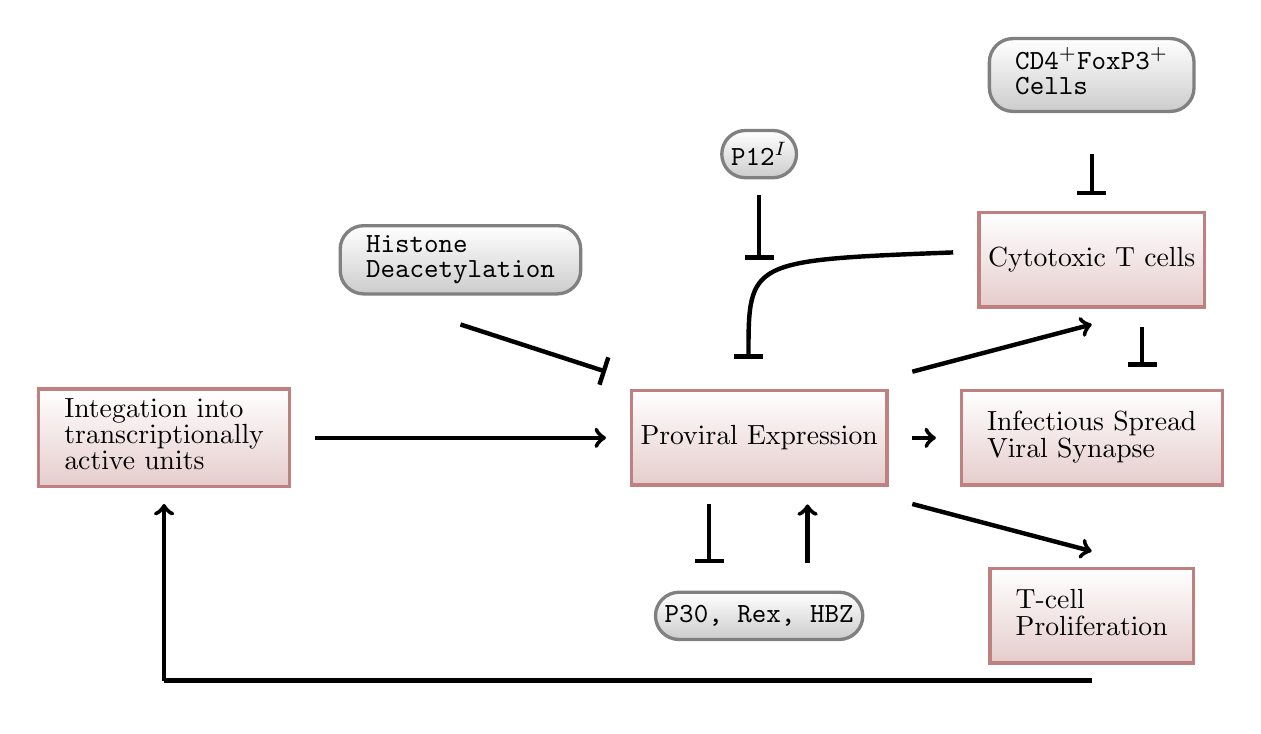
\begin{tikzpicture}[nonterminal/.style={
	rectangle,
	minimum size=12mm,
	very thick,
	draw=red!50!black!50, 
	top color=white, 
	bottom color=red!50!black!20
%	font=\itshape
	},terminal/.style={
	rectangle,minimum size=6mm,rounded corners=3mm,
	very thick,draw=black!50,
	top color=white,bottom color=black!20,
	font=\ttfamily
	},point/.style={
	circle,inner sep=0pt,minimum size=2pt,fill=red
	},point1/.style={
	coordinate,thick,draw=black!50
	}
]

\matrix[row sep=2mm,column sep=3mm] {
& & & & & & & \node (atom3) [terminal] {{\renewcommand{\arraystretch}{0.75}\begin{tabular}{l} CD4$^+$FoxP3$^+$ \\ Cells \end{tabular}}};
\\
 & & & & \node (atomP12) [terminal] {P12$^I$}; & & & \node (POSP) [point1] {.}; \\
 & & & & \node (POSY) [point1] {.}; & & & \node (POSQ) [point1] {.}; \\
% First row
 & & \node (atomHIS) [terminal] {{\renewcommand{\arraystretch}{0.75}\begin{tabular}{l} Histone \\ Deacetylation \end{tabular}}}; & & \node (POSZ) [point1] {.}; & & \node (POSO) [point1] {.}; & \node (atomCTL) [nonterminal] {Cytotoxic T cells}; \\
 & & \node (POSI) [point1] {.}; & & & & & \node (POSF) [point1] {.}; \\
 & & & & & & & \\
 & & & & & & & \\
 & & & \node (POSJ) [point1] {.}; & \node (POSN) [point1] {.}; & \node (POSE) [point1] {.}; & & \\
% Second row
\node (atom1) [nonterminal] {{\renewcommand{\arraystretch}{0.75}\begin{tabular}{l} Integation into \\ transcriptionally \\ active units \end{tabular}}}; & \node (POSA) [point1] {.}; & & \node (POSB) [point1] {.}; & \node (atom2) [nonterminal] {Proviral Expression}; & \node (POSC) [point1] {.}; & \node (POSD) [point1] {.}; & \node (atom3) [nonterminal] {{\renewcommand{\arraystretch}{0.75}\begin{tabular}{l} Infectious Spread \\ Viral Synapse \end{tabular}}};\\
\node (POSM) [point1] {.}; & & & & \node (POSR) [point1] {.}; & \node (POSG) [point1] {.}; & & \\
 & & & & & & & \\
 & & & & & & & \\
 & & & & \node (POSS) [point1] {.}; & & & \node (POSH) [point1] {.}; \\
% Third row
 & & & & \node (atomProt) [terminal] {P30, Rex, HBZ}; & & & \node (atomProl) [nonterminal] {{\renewcommand{\arraystretch}{0.75}\begin{tabular}{l} T-cell \\ Proliferation \end{tabular}}};\\
\node (POSK) [point1] {.}; & & & & & & & \node (POSL) [point1] {.}; \\
\\
};

%(x,y)
\draw[-|, ultra thick] (4.1,1.45) .. controls (1.5,1.35) .. (1.5,0.1);
\draw[ultra thick]	(POSA) edge[->] (POSB);
\draw[ultra thick]	(POSC) edge[->] (POSD);
\draw[ultra thick]	(POSE) edge[->] (POSF);
\draw[ultra thick]	(POSG) edge[->] (POSH);
\draw[ultra thick]	(POSI) edge[-|] (POSJ);
\draw[ultra thick]	(POSK) edge[-] (POSL);
\draw[ultra thick]	(POSK) edge[->] (POSM);
\draw[ultra thick]	(POSP) edge[-|] (POSQ);
\draw[ultra thick]	(POSY) edge[-|] (POSZ);
\draw[-|, ultra thick] (1,-1.75) -- (1,-2.5);
\draw[<-, ultra thick] (2.25,-1.75) -- (2.25,-2.5);
\draw[-|, ultra thick] (6.5,0.5) -- (6.5,0);

\end{tikzpicture}

\end{sideways}
\end{center}
\caption[The persistence of HTLV-I \emph{in vivo}]{The persistence of HTLV-I \emph{in vivo}. The stimulatory and inhibitory factors controlling HTLV-I proliferation (C.~Bangham, pers.~comm.).}
\label{chapter8/HTLVpers}
\end{table}

%%%%%%%%%%%%%%%%%%%%%%%%%%%%%%%%%%%%%%%%%%%%%%%%%%%%%%%%%%%%%%%%%%%%%%%%%%%%%%%%%%%%%%%%%%%%%%%%%%%%
%%%%%%%%%%%%%%%%%%%%%%%%%%%%%%%%%%%%%%%%%%%%%%%%%%%%%%%%%%%%%%%%%%%%%%%%%%%%%%%%%%%%%%%%%%%%%%%%%%%%